\documentclass[11pt,a4paper]{article}
\usepackage[T1]{fontenc}
\usepackage[utf8]{inputenc}
\usepackage{lmodern}
\usepackage[margin=2.2cm]{geometry}
\usepackage{amsmath,amssymb}
\usepackage{graphicx}
\usepackage{booktabs}
\usepackage{array}
\usepackage{siunitx}
\usepackage[font=small,labelfont=bf]{caption}
\usepackage{microtype}
\usepackage{xcolor}
\usepackage[colorlinks=true,linkcolor=blue!50!black,citecolor=blue!50!black,urlcolor=blue!50!black]{hyperref}
\usepackage{float}
\usepackage{enumitem}
\setlist{itemsep=3pt,topsep=4pt}
\sisetup{group-separator={,},group-minimum-digits=4,exponent-product=\times}
\renewcommand{\arraystretch}{1.12}

\title{\textbf{GPU (CUDA) versus CPU (TreeCorr) for the matter\\ two- and three-point correlation functions}\\[4pt]
\large Speed and precision comparison of \texttt{gpucorr} and TreeCorr 5.1.4}
\author{}
\date{GPU: NVIDIA GeForce RTX 4070 Laptop GPU \quad CPU: Intel64 Family 6 Model 183 Stepping 1, GenuineIntel, 32 threads}

\begin{document}
\maketitle

\section*{Summary}
\begin{itemize}
\item \textbf{Speed.} The complete estimator set (DD, DR, RR, DDD, DRR, RDD, RRR) with $N_\mathrm{data}=\num{10000}$ and $N_\mathrm{rand}=\num{500000}$ runs in \textbf{\SI{26.2}{min}} on the GPU. TreeCorr\textquotesingle s accurate tree algorithm (\texttt{triangle}, default \texttt{bin\_slop}) would need $\sim$\SI{57.6}{h} (extrapolated), about 132$\times$ longer; exact TreeCorr (\texttt{bin\_slop=0}) costs the same. TreeCorr\textquotesingle s default \texttt{multipole} algorithm is 4--14$\times$ slower than the GPU up to $N_\mathrm{rand}=\num{200000}$ and about as fast at \num{500000}, but it is not correct in 3D (next items).
\item \textbf{Precision.} The GPU counts every pair and triangle. Against exact TreeCorr (\texttt{bin\_slop=0}, \texttt{algo=triangle}) on the real catalogs every term agrees bin by bin in the Euclidean metric ($\Delta\xi=\num{0}$, $\Delta\zeta=\num{0}$); mean columns agree to $\sim\num{1e-6}$ (mixed precision) or \numrange{1e-12}{1e-15} (double precision).
\item \textbf{Periodic box.} Totals, $\phi$-marginals and $d_2\leftrightarrow d_3$-symmetrised counts are identical; a fraction $\le \num{6e-04}$ of triangle rotations sits in the mirror bin $(d_3,d_2)$ because TreeCorr\textquotesingle s 3D orientation rule is ambiguous for triangles crossing the box edge (Sec.~\ref{sec:orient}).
\item \textbf{TreeCorr default in 3D.} The default LogSAS algorithm (\texttt{multipole}) does not reproduce the 3D opening-angle distribution: median per-bin error 32\,\% versus 0.15\,\% for the \texttt{triangle} algorithm (Sec.~\ref{sec:mp3d}).
\item \textbf{Legendre mode (optional).} \texttt{gpu\_method: legendre} computes the Slepian--Eisenstein multipoles exactly (\num{4e-16} agreement with brute force). At $N_\mathrm{rand}=\num{500000}$ the 3PCF takes \SI{65.7}{s} with $\ell_\mathrm{max}=10$ instead of \SI{26.1}{min} for exact binned counting (24$\times$ faster); $\phi$-binned values reconstructed from it agree with exact within the shot noise (Sec.~\ref{sec:legendre}).
\end{itemize}

\section{Setup}
\paragraph{Data and binning.} \texttt{input/data.data} (\num{10000} points, unit weights) and
\texttt{input/random.txt} (\num{500000} points) in a periodic box of side $L=1000$. As in
\texttt{p2pcfconfig.yaml} and \texttt{p3pcfconfig.yaml}: 50 logarithmic bins in $50\le r<150$ and,
for the 3PCF (\texttt{LogSAS}), 50 bins in the opening angle $\phi\in[0,\pi)$.

\paragraph{Estimators.} Landy--Szalay $\xi=(DD-2DR+RR)/RR$ and the full three-point estimator
\begin{equation}
  \zeta(d_2,d_3,\phi)=\frac{DDD-RDD+DRR-RRR}{RRR},
\end{equation}
with TreeCorr's normalisation factors. Both backends use TreeCorr's own \texttt{calculateXi},
\texttt{calculateZeta} and \texttt{write}; only the pair/triangle accumulation differs.

\paragraph{Configuration.} The same config files drive every method:
\texttt{backend: cpu|cuda}, and on the GPU \texttt{gpu\_method: exact|legendre} with
\texttt{gpu\_lmax}, \texttt{gpu\_precision: mixed|double} and \texttt{max\_vram\_gb}.

\begin{table}[htbp]
\centering
\small
\caption{Compared methods.}
\label{tab:methods}
\begin{tabular}{>{\raggedright\arraybackslash}p{0.25\textwidth}>{\raggedright\arraybackslash}p{0.45\textwidth}>{\raggedright\arraybackslash}p{0.2\textwidth}}
\toprule
Backend / method & Algorithm & Approximation \\
\midrule
GPU, exact (\texttt{backend: cuda}) & periodic cell list; every candidate tested with TreeCorr\textquotesingle s leaf formulas; fp32 geometry with fp64 recheck near bin edges (mixed) or all fp64 (double) & none \\
GPU, Legendre (\texttt{gpu\_method: legendre}) & spherical-harmonic multipoles $a_{\ell m}$ + cuBLAS products (Slepian \& Eisenstein 2015) & none for $\ell\le\ell_\mathrm{max}$; $\phi$ bins truncated \\
CPU, TreeCorr default & ball tree, \texttt{bin\_slop}$\approx1$ (2PCF); \texttt{multipole} (3PCF) & cells accepted whole; incorrect $\phi$ in 3D \\
CPU, TreeCorr triangle & ball tree, default \texttt{bin\_slop}, \texttt{triangle} & cells accepted whole ($\sim$0.1\,\%) \\
CPU, TreeCorr exact & ball tree, \texttt{bin\_slop=0}, \texttt{triangle} & none (scientific reference) \\
\bottomrule
\end{tabular}
\end{table}

\section{Speed}
\begin{figure}[htbp]
\centering
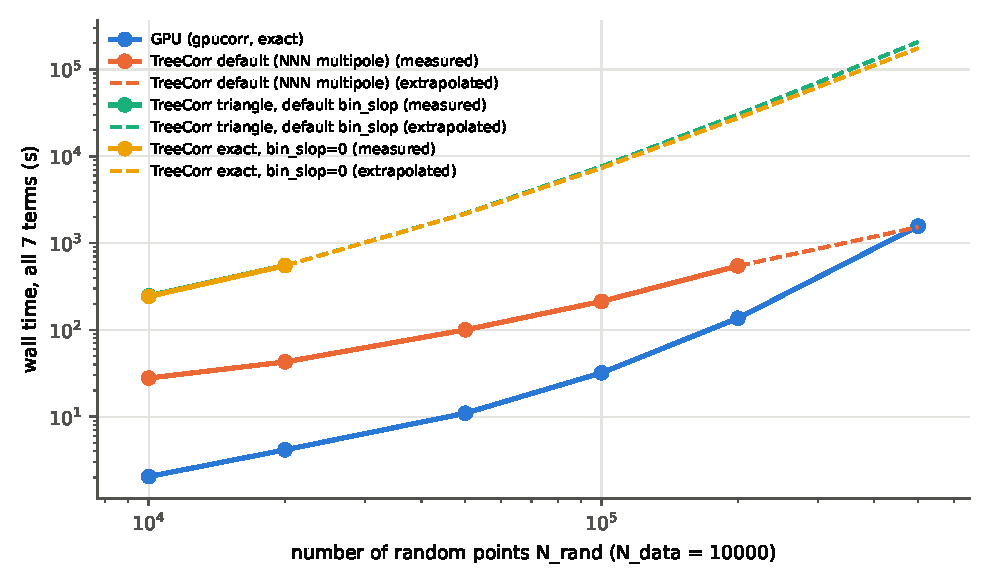
\includegraphics[width=0.9\textwidth]{fig_scaling.pdf}
\caption{Wall time of all seven terms versus the number of randoms. Solid: measured; dashed:
per-term power-law extrapolation beyond the \SI{600}{s} CPU cap. The TreeCorr \texttt{triangle}
and exact curves coincide.}
\label{fig:scaling}
\end{figure}

\begin{table}[htbp]
\centering
\small
\caption{Wall time of all seven terms ($N_\mathrm{data}=\num{10000}$). $^\ast$Exceeded the \SI{600}{s} CPU cap: extrapolated term by term with power laws fitted to the measured sizes (two sizes for the triangle/exact modes, so order-of-magnitude). Speed-up is relative to CPU triangle.}
\label{tab:speed}
\begin{tabular}{rrrrrr}
\toprule
$N_\mathrm{rand}$ & GPU exact & CPU default & CPU triangle & CPU exact & speed-up \\
\midrule
\num{10000} & \SI{2.04}{s} & \SI{27.9}{s} & \SI{4.1}{min} & \SI{4.1}{min} & 121$\times$ \\
\num{20000} & \SI{4.16}{s} & \SI{42.8}{s} & \SI{9.2}{min} & \SI{9.2}{min} & 133$\times$ \\
\num{50000} & \SI{11.0}{s} & \SI{100.2}{s} & $\sim$\SI{36.6}{min}$^\ast$ & $\sim$\SI{36.3}{min}$^\ast$ & $\sim$200$\times$ \\
\num{100000} & \SI{32.0}{s} & \SI{3.6}{min} & $\sim$\SI{2.1}{h}$^\ast$ & $\sim$\SI{2.0}{h}$^\ast$ & $\sim$239$\times$ \\
\num{200000} & \SI{2.3}{min} & \SI{9.1}{min} & $\sim$\SI{8.4}{h}$^\ast$ & $\sim$\SI{7.7}{h}$^\ast$ & $\sim$222$\times$ \\
\num{500000} & \SI{26.2}{min} & $\sim$\SI{25.5}{min}$^\ast$ & $\sim$\SI{57.6}{h}$^\ast$ & $\sim$\SI{48.8}{h}$^\ast$ & $\sim$132$\times$ \\
\bottomrule
\end{tabular}
\end{table}

At fixed box volume the number of triangles grows as $N^3$, so RRR dominates at large
$N_\mathrm{rand}$ (Fig.~\ref{fig:terms}). The GPU sustains $\sim\num{8e9}$ neighbour pairs per
second at the density of the full random catalogue. TreeCorr's \texttt{multipole} algorithm
scales almost linearly in $N$, which is why it overtakes exact counting at $N_\mathrm{rand}\approx\num{500000}$.
As Sec.~\ref{sec:mp3d} shows, however, its result is incorrect for 3D catalogues.

\begin{figure}[htbp]
\centering
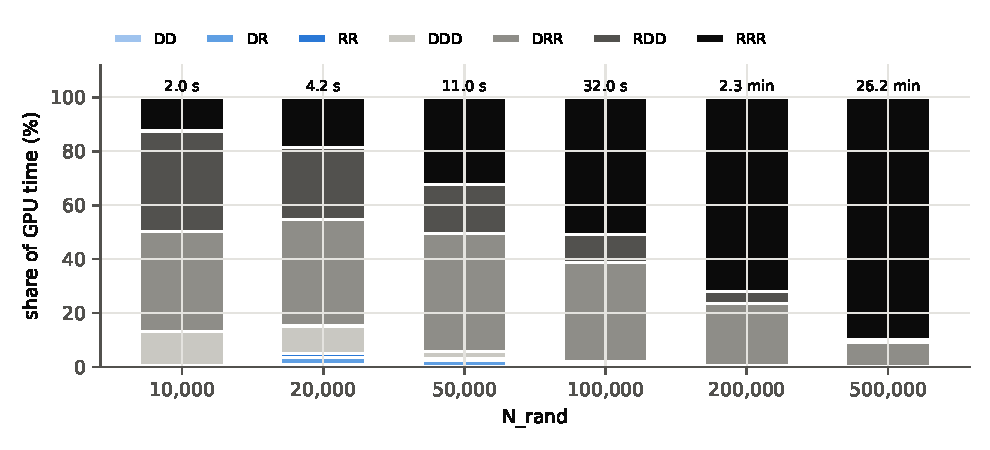
\includegraphics[width=0.88\textwidth]{fig_terms.pdf}
\caption{Share of the GPU time spent in each term; the total is printed above each bar.}
\label{fig:terms}
\end{figure}

\begin{table}[htbp]
\centering
\small
\caption{GPU time per term in seconds, peak memory and number of memory batches. The \num{200000} peak was recorded before a memory-budget fix; with the fix RRR peaks at \SI{4.2}{GB} with unchanged time.}
\label{tab:terms}
\begin{tabular}{rrrrrrrrrrr}
\toprule
$N_\mathrm{rand}$ & DD & DR & RR & DDD & DRR & RDD & RRR & total & VRAM [MiB] & batches \\
\midrule
\num{10000} & \num{0.00} & \num{0.01} & \num{0.00} & \num{0.25} & \num{0.76} & \num{0.76} & \num{0.26} & \num{2.0} & \num{102} & 6 \\
\num{20000} & \num{0.03} & \num{0.11} & \num{0.07} & \num{0.42} & \num{1.64} & \num{1.12} & \num{0.77} & \num{4.2} & \num{253} & 6 \\
\num{50000} & \num{0.03} & \num{0.25} & \num{0.06} & \num{0.30} & \num{4.80} & \num{1.99} & \num{3.53} & \num{11.0} & \num{1086} & 6 \\
\num{100000} & \num{0.03} & \num{0.18} & \num{0.18} & \num{0.26} & \num{11.74} & \num{3.40} & \num{16.25} & \num{32.0} & \num{3707} & 6 \\
\num{200000} & \num{0.03} & \num{0.25} & \num{0.49} & \num{0.26} & \num{30.92} & \num{6.13} & \num{98.28} & \num{136.4} & \num{7784} & 12 \\
\num{500000} & \num{0.01} & \num{0.25} & \num{2.86} & \num{0.25} & \num{142.58} & \num{14.37} & \num{1409.86} & \num{1570.2} & \num{4339} & 53 \\
\bottomrule
\end{tabular}
\end{table}

\paragraph{Bounded memory.} Re-running $N_\mathrm{rand}=\num{50000}$ with \texttt{max\_vram\_gb: 0.5} used 13 batches instead of 6 and peaked at \SI{331}{MiB} instead of \SI{1049}{MiB}; all counts were identical and $\max|\Delta\zeta|=\num{0}$ (\SI{10.7}{s} vs \SI{10.9}{s}). Results are independent of the memory budget, so the same run fits a \SI{12}{GB} Colab GPU or any smaller card.

\section{Precision of the exact GPU method}
\subsection{Independent brute force}
The reference applies TreeCorr's leaf-level formulas directly to every triple and shares no code
with the GPU implementation.

\begin{table}[htbp]
\centering
\small
\caption{GPU vs an independent NumPy brute force (2,000 uniform points, auto NNN). $\Delta$ = maximum relative difference of the bin means.}
\label{tab:p1}
\begin{tabular}{llrrrrrr}
\toprule
metric & precision & rotations & bins differ & $\Delta\bar d_1$ & $\Delta\bar d_2$ & $\Delta\bar\phi$ & fp64 rechecks \\
\midrule
Euclidean & mixed & \num{561876} & 0 & \num{9.4e-07} & \num{4.1e-09} & \num{6.9e-06} & \num{193} \\
Euclidean & double & \num{561876} & 0 & \num{2.0e-12} & \num{8.9e-15} & \num{5.0e-12} & \num{561876} \\
Periodic & mixed & \num{733344} & 0 & \num{1.0e-06} & \num{4.7e-09} & \num{6.9e-06} & \num{268} \\
Periodic & double & \num{733344} & 0 & \num{2.0e-12} & \num{8.9e-15} & \num{5.0e-12} & \num{733344} \\
\bottomrule
\end{tabular}
\end{table}

\subsection{TreeCorr exact on the real catalogues}
\begin{table}[htbp]
\centering
\small
\caption{Euclidean metric: GPU vs exact TreeCorr (subsample \num{2000} data, \num{4000} randoms). For NNN the count column is the difference of the totals. $\max|\Delta\xi|$: GPU \num{0}, TreeCorr default \num{4.9e-03}. $\max|\Delta\zeta|$ (bins with RRR $\ge100$): GPU \num{0}; from $d_2\leftrightarrow d_3$-symmetrised counts \num{0}; TreeCorr default (multipole) \num{2.95}.}
\label{tab:p2euc}
\begin{tabular}{lrrrrrr}
\toprule
term & $|\Delta$count$|$ & $\Delta w$ (rel) & $\Delta\bar r$ (rel) & bins differ & $\sum|\Delta n_\mathrm{tri}|$ & sym.\ bins differ \\
\midrule
DD & 0 & \num{0} & \num{1.8e-15} & --- & --- & --- \\
DR & 0 & \num{0} & \num{5.4e-15} & --- & --- & --- \\
RR & 0 & \num{0} & \num{2.9e-15} & --- & --- & --- \\
DDD & 0 & --- & --- & 0 & 0 & 0 \\
DRR & 0 & --- & --- & 0 & 0 & 0 \\
RDD & 0 & --- & --- & 0 & 0 & 0 \\
RRR & 0 & --- & --- & 0 & 0 & 0 \\
\bottomrule
\end{tabular}
\end{table}

\begin{table}[htbp]
\centering
\small
\caption{Periodic metric: GPU vs exact TreeCorr (subsample \num{2000} data, \num{4000} randoms). For NNN the count column is the difference of the totals. $\max|\Delta\xi|$: GPU \num{0}, TreeCorr default \num{3.4e-03}. $\max|\Delta\zeta|$ (bins with RRR $\ge100$): GPU \num{0.08}; from $d_2\leftrightarrow d_3$-symmetrised counts \num{0}; TreeCorr default (multipole) \num{2.65}.}
\label{tab:p2per}
\begin{tabular}{lrrrrrr}
\toprule
term & $|\Delta$count$|$ & $\Delta w$ (rel) & $\Delta\bar r$ (rel) & bins differ & $\sum|\Delta n_\mathrm{tri}|$ & sym.\ bins differ \\
\midrule
DD & 0 & \num{0} & \num{1.4e-15} & --- & --- & --- \\
DR & 0 & \num{0} & \num{5.9e-15} & --- & --- & --- \\
RR & 0 & \num{0} & \num{3.8e-15} & --- & --- & --- \\
DDD & 0 & --- & --- & 838 & 838 & 0 \\
DRR & 0 & --- & --- & 1232 & 1238 & 0 \\
RDD & 0 & --- & --- & 500 & 502 & 0 \\
RRR & 0 & --- & --- & 1142 & 1154 & 0 \\
\bottomrule
\end{tabular}
\end{table}

\section{Interpretation}
\paragraph{Counts and $\zeta$.} The integer counts are exact in both GPU precisions. With unit
weights the weights and $\zeta$, which depend only on them, are exact as well. Agreement with
exact TreeCorr is therefore bitwise in the Euclidean metric.

\paragraph{Mean columns.} In the default \emph{mixed} precision, $\bar d_1,\dots,\bar\phi$ are
accumulated from fp32 geometry ($\sim\num{1e-6}$ relative). \texttt{gpu\_precision: double}
evaluates every triangle with fp64 TreeCorr formulas and sums in exact 64-bit fixed point
(\numrange{1e-12}{1e-15}), at roughly $1/10$--$1/20$ of the speed on consumer GPUs.

\paragraph{Periodic orientation.}\label{sec:orient} TreeCorr labels $d_2/d_3$ with
$\operatorname{sign}[(\mathbf r_{13}\times\mathbf r_{12})\cdot\mathbf p_1]$, a dot product with the
\emph{absolute} position of a vertex. In the auto-correlation it evaluates this once, at whichever
vertex its tree traversal reaches first, and reuses it for all three rotations. For triangles that
straddle the periodic boundary the sign differs between vertices (\num{45486} of \num{733344} rotations in the
brute-force test). TreeCorr's own assignment therefore depends on traversal order. \texttt{gpucorr}
always applies the test at $P_1$. This only moves triangles between the mirror bins $(k_2,k_3)$ and
$(k_3,k_2)$, which for a statistically isotropic box is pure relabelling.

\subsection{TreeCorr's default 3PCF algorithm in 3D}\label{sec:mp3d}
\begin{figure}[htbp]
\centering
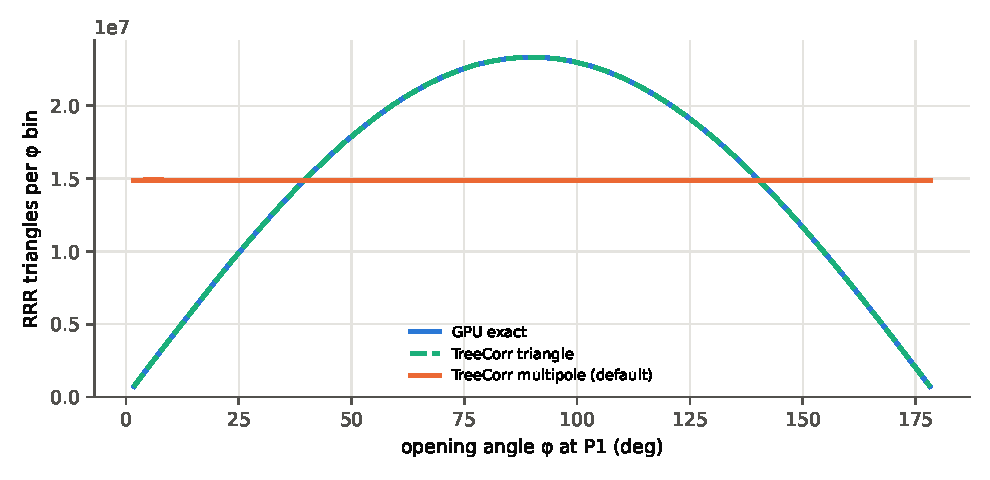
\includegraphics[width=0.85\textwidth]{fig_multipole.pdf}
\caption{$\phi$-distribution of RRR for \num{20000} randoms from \texttt{input/random.txt} (periodic
box), summed over all $(d_2,d_3)$. For uniform randoms the true distribution follows $\sin\phi$
(GPU exact and TreeCorr \texttt{triangle} coincide). TreeCorr's \texttt{multipole} algorithm returns an
essentially flat distribution.}
\label{fig:mp}
\end{figure}

\begin{table}[htbp]
\centering
\small
\caption{TreeCorr\textquotesingle s default LogSAS algorithm in 2D and 3D (relative differences, bins with $>300$ triangles).}
\label{tab:mp}
\begin{tabular}{llrrr}
\toprule
catalog & reference & multipole: median $|\Delta|$ & multipole: $\phi$-marg.\ max & triangle: median $|\Delta|$ \\
\midrule
2D, $N=\num{6000}$ & TreeCorr triangle & \num{0.02} & \num{0.01} & (reference) \\
3D, $N=\num{20000}$ & GPU exact & \num{0.32} & \num{19.76} & \num{1.7e-03} \\
\bottomrule
\end{tabular}
\end{table}

In 3D the median per-bin deviation of the multipole algorithm from exact counting is 32\,\% (triangle algorithm: 0.15\,\%), while the total over all bins is still correct (\num{3.0e-06}). Raising \texttt{max\_n} to 200 does not change it, so this is not truncation. The multipole path should therefore not be used for 3D box 3PCFs with TreeCorr 5.1.4.
Use \texttt{algo: triangle} on the CPU, or either GPU method.

%%LEG-BEGIN
\section{Legendre multipole mode (Slepian \& Eisenstein) versus exact counting}\label{sec:legendre}
\paragraph{Method.} With \texttt{gpu\_method: legendre}, \texttt{gpucorr} computes for every
centre $c$ and radial bin $k$
\begin{equation}
  a_{\ell m}(c,k)=\sum_{j\in k} w_j\,Y_{\ell m}(\hat{\mathbf r}_{cj}),
\end{equation}
using fully normalised associated Legendre functions with a stable three-term recursion. The
addition theorem then gives the Legendre moments of the triangle counts as a matrix product over
all centres:
\begin{equation}
  M_\ell(k_2,k_3)=\sum_c w_c\!\!\sum_{\substack{j\in k_2,\,l\in k_3\\ j\neq l}}\!\! w_j w_l\,P_\ell(\cos\phi_{jl})
  =\frac{4\pi}{2\ell+1}\sum_c w_c\Big[a_{\ell0}a_{\ell0}^{*}+2\,\mathrm{Re}\sum_{m>0}a_{\ell m}(k_2)\,a_{\ell m}^{*}(k_3)\Big]-\delta_{k_2k_3}\,S,
\end{equation}
where $S$ removes the self-pairs. The cost scales as $N\,n\,\ell_\mathrm{max}^2$ instead of
$N\,n^2$. The multipoles of every term are written to \texttt{<file>\_legendre.txt}, with
$\zeta_\ell=Z_\ell/(RRR_0 f)$ so that $\zeta(\phi)\simeq\sum_\ell(2\ell+1)\,\zeta_\ell\,P_\ell(\cos\phi)$.
The usual TreeCorr file receives $\phi$ bins reconstructed from the truncated series,
\begin{equation}
  N(\phi_a<\phi<\phi_b)=\sum_{\ell\le\ell_\mathrm{max}}\frac{2\ell+1}{2}\,M_\ell\int_{\cos\phi_b}^{\cos\phi_a}P_\ell(\mu)\,d\mu,
\end{equation}
symmetric in $d_2\leftrightarrow d_3$ (the method has no 3D orientation).

\paragraph{Correctness.} Against an independent NumPy brute force of $\sum P_\ell(\cos\phi)$ over
every triangle (\num{2000} points, $\ell\le12$), the multipoles agree to \num{4e-16} in double
precision and \num{3e-7} in mixed precision, in both metrics. On the real catalogues the monopole
equals the exact triangle total of every term (largest relative difference \num{0}).

\subsection{Comparison in \texorpdfstring{$\phi$}{phi} bins}
\begin{table}[htbp]
\centering
\small
\caption{$\phi$-binned reconstruction from the Legendre mode vs symmetrised exact counts (\num{10000} data, \num{50000} randoms, periodic box). $\sigma_\zeta$: shot-noise error of the exact $\zeta$ (median \num{0.046}; rms $\zeta$ = \num{0.095}).}
\label{tab:legbin}
\begin{tabular}{rrrrrr}
\toprule
$\ell_\mathrm{max}$ & RRR median $|\Delta|$ & RRR $\phi$-marg.\ max & DDD median $|\Delta|$ & rms $\Delta\zeta$ & rms $\Delta\zeta/\sigma_\zeta$ \\
\midrule
2 & \num{2.5e-03} & \num{6.0e-03} & \num{0.02} & \num{0.092} & \num{0.96} \\
4 & \num{2.5e-03} & \num{5.3e-03} & \num{0.02} & \num{0.090} & \num{0.94} \\
6 & \num{2.4e-03} & \num{4.5e-03} & \num{0.02} & \num{0.088} & \num{0.92} \\
8 & \num{2.3e-03} & \num{3.4e-03} & \num{0.02} & \num{0.086} & \num{0.90} \\
10 & \num{2.3e-03} & \num{2.2e-03} & \num{0.02} & \num{0.084} & \num{0.87} \\
16 & \num{2.1e-03} & \num{3.9e-03} & \num{0.02} & \num{0.079} & \num{0.81} \\
24 & \num{1.9e-03} & \num{2.4e-03} & \num{0.01} & \num{0.068} & \num{0.72} \\
32 & \num{1.6e-03} & \num{7.9e-04} & \num{0.01} & \num{0.059} & \num{0.63} \\
49 & \num{1.2e-03} & \num{4.8e-04} & \num{9.4e-03} & \num{0.041} & \num{0.45} \\
\bottomrule
\end{tabular}
\end{table}

The per-bin differences are of the size of the Poisson noise of the exact counts. A truncated
Legendre series removes the high-$\ell$ part of that noise, so $\Delta\zeta\approx1\sigma$ at small
$\ell_\mathrm{max}$, decreasing towards $\ell_\mathrm{max}=49$ (50 $\phi$ bins). The difference is
mostly noise filtering rather than bias: the smooth angular signal is captured already at
$\ell_\mathrm{max}\approx10$ (Fig.~\ref{fig:legzeta}).

\begin{figure}[htbp]
\centering
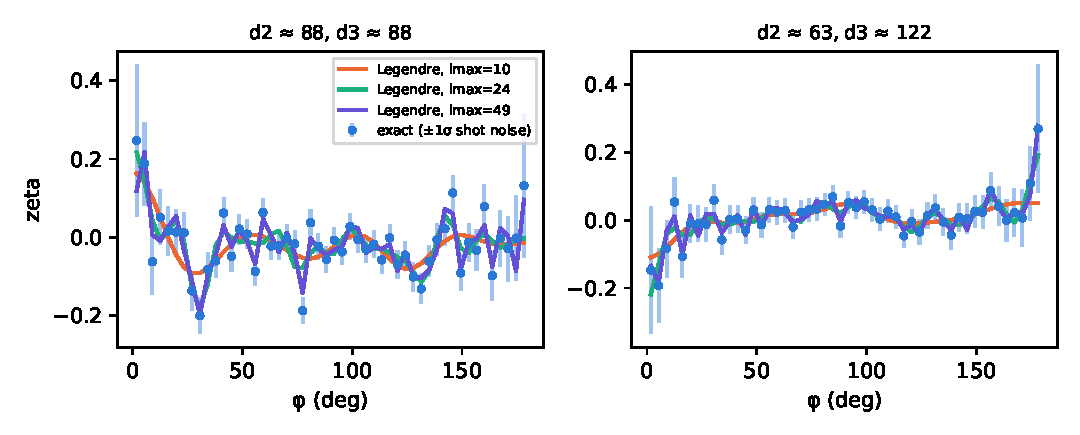
\includegraphics[width=\textwidth]{fig_leg_zeta.pdf}
\caption{$\zeta(\phi)$ in two $(d_2,d_3)$ bins: exact counting with shot-noise error bars, and
reconstructions from the Legendre mode.}
\label{fig:legzeta}
\end{figure}

\begin{figure}[htbp]
\centering
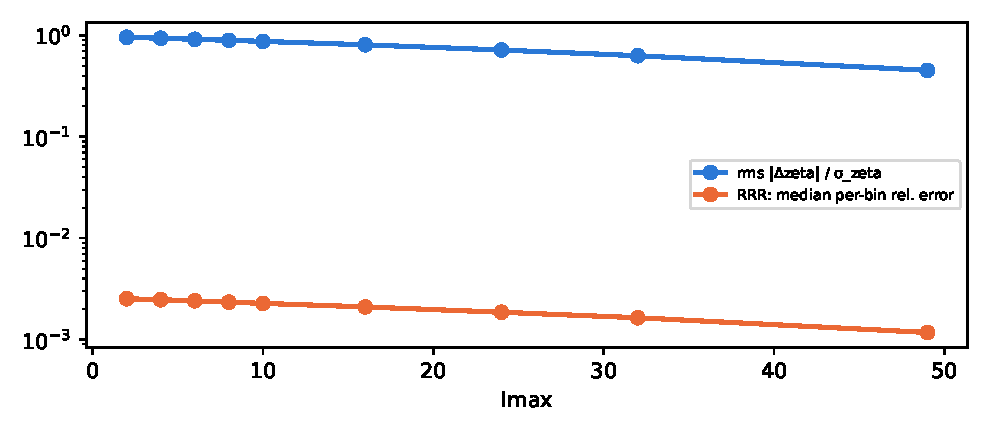
\includegraphics[width=0.8\textwidth]{fig_leg_conv.pdf}
\caption{Convergence of the $\phi$-binned reconstruction with $\ell_\mathrm{max}$.}
\label{fig:legconv}
\end{figure}

\subsection{Comparison in multipole space}
\begin{table}[htbp]
\centering
\small
\caption{Multipoles $\zeta_\ell$: Legendre mode vs projection of the exact $\phi$-binned counts onto $P_\ell$ (rms over $(d_2,d_3)$ bins, relative to rms $\zeta_\ell$). The difference shrinks as the exact binning is refined.}
\label{tab:legml}
\begin{tabular}{rrrr}
\toprule
$\ell$ & rms $\zeta_\ell$ & rel.\ $\Delta$ (50 $\phi$ bins) & rel.\ $\Delta$ (200 $\phi$ bins) \\
\midrule
0 & \num{1.6e-02} & \num{0} & --- \\
1 & \num{5.5e-03} & \num{2.4e-02} & \num{6.3e-03} \\
2 & \num{4.2e-03} & \num{4.6e-02} & \num{1.0e-02} \\
3 & \num{3.4e-03} & \num{6.3e-02} & --- \\
4 & \num{3.3e-03} & \num{7.3e-02} & \num{1.8e-02} \\
5 & \num{2.9e-03} & \num{8.8e-02} & --- \\
6 & \num{2.6e-03} & \num{1.1e-01} & \num{2.9e-02} \\
7 & \num{2.4e-03} & \num{1.3e-01} & --- \\
8 & \num{2.2e-03} & \num{1.5e-01} & \num{3.6e-02} \\
9 & \num{2.0e-03} & \num{1.9e-01} & --- \\
10 & \num{2.0e-03} & \num{1.8e-01} & \num{4.9e-02} \\
\bottomrule
\end{tabular}
\end{table}

The monopole agrees to \num{1e-5}. The higher multipoles differ by an amount set by the
\emph{exact} method's $\phi$-binning: with 200 instead of 50 bins the difference falls about
fourfold and converges to the Legendre values. For multipole analyses the Legendre mode is
therefore the more accurate of the two, being exact up to round-off.

\subsection{Speed}
\begin{figure}[htbp]
\centering
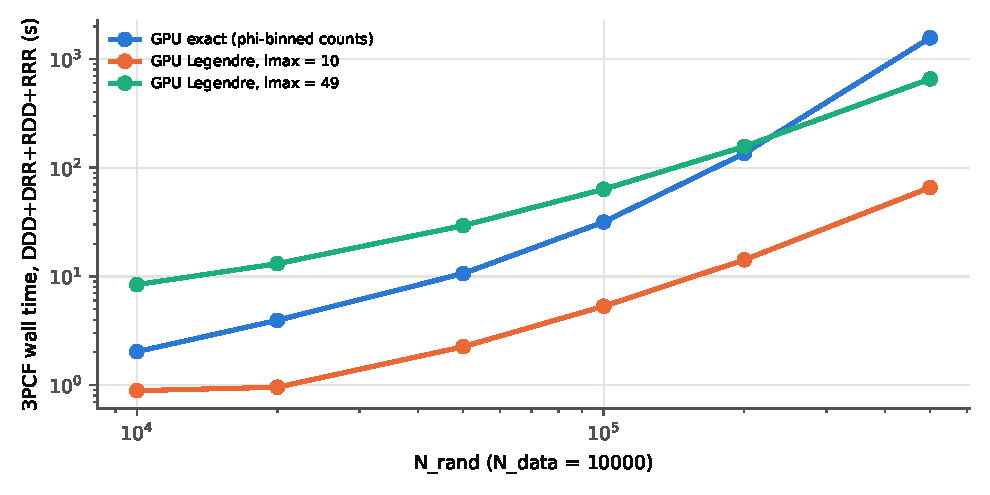
\includegraphics[width=0.85\textwidth]{fig_leg_timing.pdf}
\caption{3PCF wall time of the exact and Legendre GPU methods ($N_\mathrm{data}=\num{10000}$).}
\label{fig:legtime}
\end{figure}

\begin{table}[htbp]
\centering
\small
\caption{3PCF wall time (DDD, DRR, RDD, RRR) of the two GPU methods.}
\label{tab:legtime}
\begin{tabular}{rrrrrr}
\toprule
$N_\mathrm{rand}$ & exact & Legendre $\ell_\mathrm{max}=10$ & speed-up & Legendre $\ell_\mathrm{max}=49$ & speed-up \\
\midrule
\num{10000} & \SI{2.03}{s} & \SI{0.89}{s} & 2.3$\times$ & \SI{8.40}{s} & 0.2$\times$ \\
\num{20000} & \SI{3.95}{s} & \SI{0.96}{s} & 4.1$\times$ & \SI{13.1}{s} & 0.3$\times$ \\
\num{50000} & \SI{10.6}{s} & \SI{2.26}{s} & 4.7$\times$ & \SI{29.4}{s} & 0.4$\times$ \\
\num{100000} & \SI{31.7}{s} & \SI{5.32}{s} & 6.0$\times$ & \SI{63.4}{s} & 0.5$\times$ \\
\num{200000} & \SI{2.3}{min} & \SI{14.2}{s} & 9.5$\times$ & \SI{2.6}{min} & 0.9$\times$ \\
\num{500000} & \SI{26.1}{min} & \SI{65.7}{s} & 23.9$\times$ & \SI{10.9}{min} & 2.4$\times$ \\
\bottomrule
\end{tabular}
\end{table}

The Legendre cost grows with the number of neighbour pairs ($\propto N n$), exact counting with the
number of triangles ($\propto N n^2$), so the advantage increases with density. At small $N$ the
fixed costs (neighbour lists, per-$\ell$ matrix products) dominate.
%%LEG-END

\section{Recommendations}
\begin{itemize}
\item Multipole analyses ($\zeta_\ell$): \texttt{backend: cuda}, \texttt{gpu\_method: legendre}
      ($\ell_\mathrm{max}\approx10$). The multipoles are exact, and at high density the method is
      much faster.
\item $\phi$-binned 3PCF: \texttt{backend: cuda} with the default \texttt{gpu\_method: exact},
      \texttt{gpu\_precision: mixed}. Counts, weights and $\zeta$ are exact; the means are good to
      \num{1e-6}.
\item When the mean columns must match TreeCorr to machine precision: \texttt{gpu\_precision: double}.
\item CPU cross-checks: \texttt{algo: triangle} (or \texttt{bin\_slop: 0} on subsamples), not the
      default \texttt{multipole} algorithm.
\item Colab or smaller GPUs: set \texttt{max\_vram\_gb}; results do not depend on it.
\end{itemize}

\paragraph{Reproduction.} \texttt{python tests/validate\_vs\_treecorr.py};
\texttt{python bench/benchmark.py}; \texttt{python tests/check\_legendre.py};
\texttt{python tests/compare\_legendre.py}; \texttt{python report/make\_report\_tex.py}.

\end{document}
